\documentclass{article} % For LaTeX2e
\usepackage{iclr2018_conference,times}
\usepackage{hyperref}
\usepackage{url}

% For table captions
\usepackage{caption}
\captionsetup[table]{skip=10pt}

% For figures and subfigures
\usepackage{graphicx}
\usepackage{subcaption}

% Disable word splitting
\tolerance=1
\emergencystretch=\maxdimen
\hyphenpenalty=10000
\hbadness=10000

\usepackage{amsmath}

\title{Stochastic Collection and Deletion of Experience Replay}
\author{Ryan Lee}

\begin{document}
\maketitle

%%%%%%%%%%%%%%%%%%%%%%%%%%%%%%%%%%%%%%%%%%%%%%%%%%%%%%%%%%%%%%%%%%%%%%%%%%%%%%%%
% ABSTRACT                                                                     %
%%%%%%%%%%%%%%%%%%%%%%%%%%%%%%%%%%%%%%%%%%%%%%%%%%%%%%%%%%%%%%%%%%%%%%%%%%%%%%%%
\begin{abstract}
\textit{Experience Replay} allows an online reinforcement learning agent to replay previous experiences to learn more about the environment. Prior works of improving Experience Replay have focused on improving the sampling method, prioritizing experiences with high TD error $\lvert \delta \rvert$. We explore different collection and deletion methods for experience replay to make the replay memory more memory-efficient. We evaluate the effectiveness of these methods with a Rainbow Deep Q Network (DQN) agent in custom stages of \textit{Sonic the Hedgehog} games provided by OpenAI.
\end{abstract}





\section{Background}
%%%%%%%%%%%%%%%%%%%%%%%%%%%%%%%%%%%%%%%%%%%%%%%%%%%%%%%%%%%%%%%%%%%%%%%%%%%%%%%%
% BACKGROUND                                                                   %
%%%%%%%%%%%%%%%%%%%%%%%%%%%%%%%%%%%%%%%%%%%%%%%%%%%%%%%%%%%%%%%%%%%%%%%%%%%%%%%%
Several Reinforcement Learning algorithms have been tested on \textit{Atari 2600} games. The first seminal result was Deep Q Network (DQN) by \cite{DQN}, which achieved superhuman results on 29 out of 49 games by using target network and experience replay. Many scholars have improved the original DQN algorithm since, notable enhancements being Double DQN by \cite{Double}, Prioritized Experience Replay by \cite{PER}, Dueling Network by \cite{DuelingDQN}, Distributional DQN by \cite{DistributionalDQN}, and Noisy Nets by \cite{NoisyNetDQN}, integrated into Rainbow DQN by \cite{Rainbow}. Among these improvements, we continue the discussion by \cite{PER} on improving experience replay.

There are three principal components to experience replay: collection, sampling, and deletion. The agent can choose which experience to remember, to use, and to forget. In the original DQN by \cite{DQN}, experiences were collected unconditionally, sampled randomly, and deleted chronologically. \cite{PER} improved sampling by prioritizing experiences with high TD error during sampling.

In this paper, we explore several algorithms to selectively collect and delete experiences.  We add a stochastic threshold for new experiences based on their TD errors $\lvert \delta \rvert$ and stochastically delete experiences in the replay memory with the change of TD errors $\Delta \lvert \delta \rvert$. We comparatively assess these algorithms with custom stages of \textit{Sonic the Hedgehog} games provided by OpenAI's \textit{Retro Contest} by \cite{Retro} with limited number of timesteps and computation time.




\section{Collection Threshold}
%%%%%%%%%%%%%%%%%%%%%%%%%%%%%%%%%%%%%%%%%%%%%%%%%%%%%%%%%%%%%%%%%%%%%%%%%%%%%%%%
% COLLECTION THRESHOLD                                                         %
%%%%%%%%%%%%%%%%%%%%%%%%%%%%%%%%%%%%%%%%%%%%%%%%%%%%%%%%%%%%%%%%%%%%%%%%%%%%%%%%
\cite{PER} identified two levels of design choices for replay memory: choosing  which experiences to store, and choosing which experiences to replay. \textit{Prioritized Experience Replay} only addressed the latter, exploring methods of experience prioritization by their TD errors. We explore the former, implementing various thresholds to collect experiences in a memory-efficient manner.

The effectiveness of \textit{Prioritized Experience Replay} stems from replaying valuable experience more frequently. With a large replay memory, prioritized sampling can replay each valuable experience sufficient number of times. However, with a replay memory too small, the agent could discard valuable experience without sufficiently replaying it. To discourage premature deletion of valuable experiences, we add a threshold to only collect experiences that are worth collecting at the expense of deleting a possibly valuable experience.

\subsection{Threshold with TD error}
To sample experiences from the collection, \cite{PER} used the TD error $\lvert \delta \rvert$. This was a particularly good choice for two reasons. First, by definition, TD error is an estimate of the difference between expected and actual reward. Thus, experiences with high TD error are unexpected experiences that the model should learn. Also, the TD error of every experience is computed to train the model, so prioritizing with TD error does not introduce extra computations.

To minimize extra computation, we also use the TD error to filter experiences. We only collect experiences with a TD error greater than some threshold. Using a different metric to estimate the value of the experience might enhance performance, but due to the time limit specified by \cite{Retro}, computing another metric for each experience would be too costly.

There are multiple candidates for the threshold. The weakest threshold is the minimum TD error of all the experiences in the replay memory (\textit{Buffer Minimum}). This threshold is too weak to meaningfully affect the collection process. The strongest threshold is the maximum TD error in the buffer (\textit{Buffer Maximum}). This threshold ignores too many experiences and thus slows the collection of new experiences. A better candidate for threshold is the average TD error of experiences in the replay memory (\textit{Buffer Average}).

To compute the average TD error, we use a moving average formula to update the mean every time a new experience is collected (Equation \ref{eqn:moving_average}). The mean should also be updated when an experience is replaced because the replay memory is full or when the TD errors are recalculated after replay (Equation \ref{eqn:error_recalc}).

\begin{equation}
\label{eqn:moving_average}
M_{n+1} := M_n + \frac{\lvert \delta_{n+1} \rvert - M_n}{n+1}
\end{equation}

\begin{equation}
\label{eqn:error_recalc}
M_{n+1} := M_n + \frac{\lvert \delta_{\text{new}} \rvert - \lvert \delta_{\text{old}} \rvert}{\text{capacity}}
\end{equation}

\subsection{Stochastic Threshold}
Although thresholds improve memory efficiency, the performance of the agent might drop because the threshold can prevent some valuable experiences from being collected and replayed. This phenomenon is mostly caused by the noise of the TD error. With a greedy threshold, a valuable experience affected by a negative noise is often discarded by the collection threshold. 

To mitigate this performance issue, we use a stochastic threshold that sometimes collects experience below the threshold. Adding stochasticity makes the threshold weaker, so we use a stronger threshold (\textit{Buffer Maximum}).

There are countless possibilities for adding stochasticity to threshold, since any monotonically increasing function with range $R \subset [0, 1]$ is a valid candidate (Figure \ref{fig:collection_prob_funcs}). We used the simplest linear probability function (Equation \ref{eqn:linear_probability}).

\begin{equation}
P(\text{Collect}(E_i)) = \min \left( \frac{\lvert \delta_i \rvert}{\lvert \delta_{\text{max}} \rvert}, 1 \right)
\label{eqn:linear_probability}
\end{equation}

\begin{figure}[!ht]
  \centering
  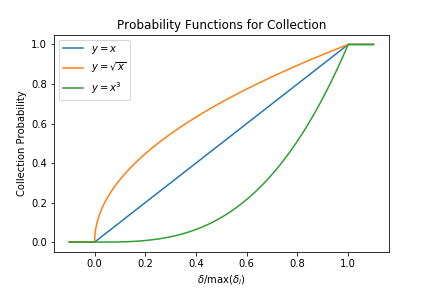
\includegraphics[width=.5\textwidth]{images/ProbabilityFunctions.png}
  \caption{Examples of polynomial collection probability functions with clipped range}
  \label{fig:collection_prob_funcs}
\end{figure}



\section{Prioritized Deletion}
%%%%%%%%%%%%%%%%%%%%%%%%%%%%%%%%%%%%%%%%%%%%%%%%%%%%%%%%%%%%%%%%%%%%%%%%%%%%%%%%
% PRIORITIZED DELETION                                                         %
%%%%%%%%%%%%%%%%%%%%%%%%%%%%%%%%%%%%%%%%%%%%%%%%%%%%%%%%%%%%%%%%%%%%%%%%%%%%%%%%
With infinite computational resources, all experience can be stored in the replay memory and learned repeatedly. In reality, the computational resources are finite, so the replay memory has a set capacity. Both \cite{DQN} and \cite{PER} deleted the oldest experience when the replay memory was full. If the replay memory is sufficiently large, all valuable experiences will be replayed sufficient times before they are deleted. However, with too small a replay memory, some crucial experience can be deleted prematurely. Thus, we prioritize experiences in the replay memory to discourage deletion of valuable experiences.

\subsection{Delta Deletion}
A natural candidate to delete is the experience with the least TD error $\lvert \delta \rvert$. However, because TD error was used for both collection and sampling, reusing this metric did not impact the performance significantly. Therefore, we also used the change of TD error $\Delta \lvert \delta \rvert$ to prioritize experiences for deletion. Although TD errors estimate the unexpectedness of an experience well, it cannot detect unlearnable experiences. An unlearnable experience with high TD error hinders learning because it is sampled often due to its high TD error without improving the model. To mitigate this issue, we use the \textit{derivative} of the TD error $\delta$ to prioritize experiences for deletion. Every time an experience is replayed from the replay memory, the TD error is updated, so the derivative can be estimated by the difference of TD errors before and after the update (Equation \ref{eqn:derivative_error}). In our implementation. experiences that have never been replayed are given high derivative values $\Delta \lvert \delta \rvert$ to ensure that all experience is replayed at least once.

\begin{equation}
\Delta \lvert \delta \rvert = \lvert \delta_{\text{old}} \rvert - \lvert \delta_{\text{new}} \rvert
\label{eqn:derivative_error}
\end{equation}

\subsection{Stochastic Deletion}
Like collection and sampling, greedy deletion leads to a performance drop due to TD error noise. Thus, we extend the stochastic argument to deletion. Unlike in prioritized sampling where high values corresponded to high probabilities, for deletion, the higher the TD error change $\Delta \lvert \delta \rvert$ is, the lower the deletion probability should be. Therefore, we use a reversed softmax function (Equation \ref{eqn:reversed_softmax}).

\begin{equation}
P(E_j) = \frac{e^{-\Delta \lvert \delta_j \rvert}}{\sum_i e^{-\Delta \lvert \delta_i \rvert}}
\label{eqn:reversed_softmax}
\end{equation}


\section{Results}
%%%%%%%%%%%%%%%%%%%%%%%%%%%%%%%%%%%%%%%%%%%%%%%%%%%%%%%%%%%%%%%%%%%%%%%%%%%%%%%%
% RESULTS                                                                      %
%%%%%%%%%%%%%%%%%%%%%%%%%%%%%%%%%%%%%%%%%%%%%%%%%%%%%%%%%%%%%%%%%%%%%%%%%%%%%%%%
The scores from the test set of the \textit{Retro Contest} had a very large variance: the same stochastic maximum threshold agent had a score difference of 3000 in Task 4 (Table \ref{table:scores}). Thus, only a limited analysis of performance is possible. Agents with stochastic collection (Figure \ref{fig:collection_performance}) or stochastic deletion (Figure \ref{fig:deletion_performance}) had a small performance increase, whereas agents with both stochastic collection and deletion had a performance drop (Figure \ref{fig:combined_performance}). Further training with different environments is needed to verify this interesting observation.


\begin{table}[!htbp]
  \centering
  \begin{tabular}{ {l}*{6}{c} }
    \hline
                                         &     \#1 &     \#2 &     \#3 &     \#4 &     \#5 & Average \\ \hline
     Baseline                            & 7740.04 & 2323.51 & 2038.93 & 5085.12 & 3268.59 & 4091.24 \\
     Baseline                            & 7662.17 & 2827.67 & 2740.57 & 5782.61 & 3339.20 & 4470.44 \\ \hline
 Minimum                                 & 7706.23 & 2569.26 & 3069.25 & 2513.12 & 3307.15 & 3833.00 \\
 BufferAverage                           & 7666.15 & 3745.61 & 1381.75 & 5005.94 & 3385.39 & 4236.97 \\
 StochasticBufferAverage                 & 7563.53 & 2660.62 & 2359.74 & 4126.60 & 3231.24 & 3988.35 \\
 StochasticMaximum                       & 7447.32 & 4030.97 & 2681.76 & 1907.79 & 2703.91 & 3754.35 \\
 StochasticMaximum                       & 7537.61 & 2970.10 & 2921.54 & 3514.32 & 2994.49 & 3987.61 \\
 StochasticMaximum                       & 7382.44 & 3739.57 & 2991.12 & 4902.19 & 3347.11 & 4472.48 \\ \hline
 MinimumDeletion                         & 7717.11 & 2583.42 & 1387.13 & 5827.83 & 3414.06 & 4185.91 \\
 StochasticDeletion                      & 7426.93 & 2711.12 & 3251.27 & 4646.53 & 3447.60 & 4296.69 \\
 StochasticDeltaDeletion                 & 7797.27 & 3423.03 & 1003.70 & 1992.22 & 3486.24 & 3540.49 \\ \hline
 StochasticMaxStochasticDeletion         & 7460.97 & 3860.93 & 2175.60 & 2426.37 & 3361.43 & 3857.06 \\
 StochasticMaxStochasticDeltaDeletion    & 7726.53 & 2638.33 & 2062.36 & 2975.46 & 3454.15 & 3771.37 \\

  \end{tabular}
  \caption{Scores from the \textit{Retro Contest}. Agents tested multiple times have multiple rows.\label{table:scores}}
  
\end{table}

We could not tune the hyperparameters for each variant of the replay memory. Thus, we used the hyperparameters in the baseline Rainbow DQN provided by \cite{Retro} (Table \ref{table:hyperparameters}). It is likely that the agents would perform better after their hyperparameters are properly tuned.

\begin{table}[!htbp]
  \centering
  \begin{tabular}{ l c }
    \hline
    Hyperparameters                            & Value                \\ \hline
    Min history to start learning              & 20K frames           \\
    Adam learning rate                         & $1 \times 10^{-4}$   \\
    Exploration $\epsilon$                     & 0.0                  \\
    Noisy Nets $\sigma_0$                      & 0.5                  \\
    Target Network Period                      & 8192 frames          \\
    Adam $\epsilon$                            & $1.5 \times 10^{-4}$ \\
    Prioritization type                        & proportional         \\
    Prioritization exponent $\omega$           & 0.5                  \\
    Prioritization importance sampling $\beta$ & 0.4                  \\
    Multi-step returns $n$                     & 3                    \\
    Distributional atoms                       & 51                   \\
    Distributional min/max values              & [-200, 200]
  \end{tabular}
  \caption{Universal hyperparameters for all agents}
  \label{table:hyperparameters}
\end{table}




\section{Conclusion}
%%%%%%%%%%%%%%%%%%%%%%%%%%%%%%%%%%%%%%%%%%%%%%%%%%%%%%%%%%%%%%%%%%%%%%%%%%%%%%%%
% CONCLUSION                                                                   %
%%%%%%%%%%%%%%%%%%%%%%%%%%%%%%%%%%%%%%%%%%%%%%%%%%%%%%%%%%%%%%%%%%%%%%%%%%%%%%%%
We could not determine if applying stochastic collection and deletion improves the replay memory due to the high variance of performance in \textit{Retro Contest}. Another assessment with a simpler environment with shorter episode lengths such as \textit{Breakout} or \textit{Pong} in \textit{Atari 2600} would produce a more conclusive result. A full grid-based hyperparameter tuning nts with stochastic collection or stochastic deletion had a small performance increase, would be too computationally extensive, but an informal tuning for hyperparameters related to the replay memory should improve the agents' performance.

There were a few more ideas in both collection and deletion that were unimplemented because they introduced new hyperparameters. For collection, a weighted average could have been a better choice since TD error $\lvert \delta \rvert$ would decrease over time. For deletion, adding a staleness factor to experiences in the replay memory would have factored both the experience's age and the change of TD error $\Delta \lvert \delta \rvert$. Another unexplored deletion method was deleting \textit{multiple} experiences even when the replay memory is not full. For every update, a batch of experience in the replay memory have their TD errors recalculated. A stochastic threshold can be used to filter out unsuitable experiences, although the threshold should be chosen carefully to maintain a reasonably sized replay memory. This has the potential of improving the agent's performance because the agent can quickly discard obsolete experiences.


%%%%%%%%%%%%%%%%%%%%%%%%%%%%%%%%%%%%%%%%%%%%%%%%%%%%%%%%%%%%%%%%%%%%%%%%%%%%%%%%
% BIBLIOGRAPHY                                                                 %
%%%%%%%%%%%%%%%%%%%%%%%%%%%%%%%%%%%%%%%%%%%%%%%%%%%%%%%%%%%%%%%%%%%%%%%%%%%%%%%%
\bibliography{iclr2018_conference}
\bibliographystyle{iclr2018_conference}



%%%%%%%%%%%%%%%%%%%%%%%%%%%%%%%%%%%%%%%%%%%%%%%%%%%%%%%%%%%%%%%%%%%%%%%%%%%%%%%%
% FIGURES                                                                      %
%%%%%%%%%%%%%%%%%%%%%%%%%%%%%%%%%%%%%%%%%%%%%%%%%%%%%%%%%%%%%%%%%%%%%%%%%%%%%%%%
\clearpage

\begin{figure*}[!ht]
    \centering
    \begin{subfigure}[t]{0.5\textwidth}
        \centering
        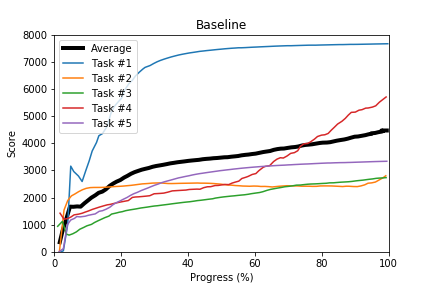
\includegraphics[width=\textwidth]{images/Baseline.png}
    \end{subfigure}%
    ~ 
    \begin{subfigure}[t]{0.5\textwidth}
        \centering
        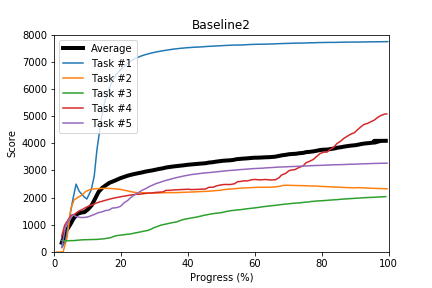
\includegraphics[width=\textwidth]{images/Baseline2.png}
    \end{subfigure}%

    \begin{subfigure}[t]{0.5\textwidth}
        \centering
        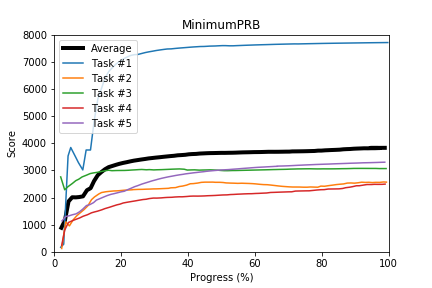
\includegraphics[width=\textwidth]{images/MinimumPRB.png}
    \end{subfigure}%
    ~
    \begin{subfigure}[t]{0.5\textwidth}
        \centering
        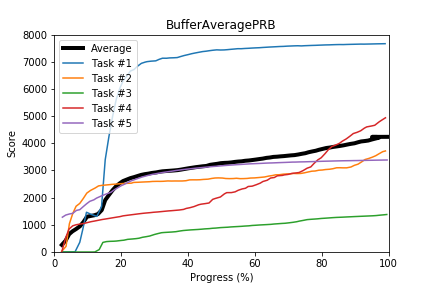
\includegraphics[width=\textwidth]{images/BufferAveragePRB.png}
    \end{subfigure}%

   \begin{subfigure}[t]{0.5\textwidth}
        \centering
        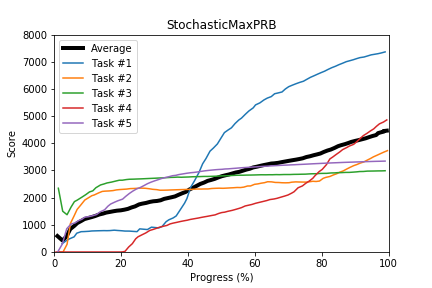
\includegraphics[width=\textwidth]{images/StochasticMaxPRB.png}
    \end{subfigure}%
	~     
    \begin{subfigure}[t]{0.5\textwidth}
        \centering
        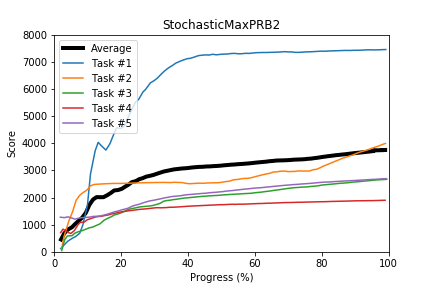
\includegraphics[width=\textwidth]{images/StochasticMaxPRB2.png}
    \end{subfigure}%
    
    \begin{subfigure}[t]{0.5\textwidth}
        \centering
        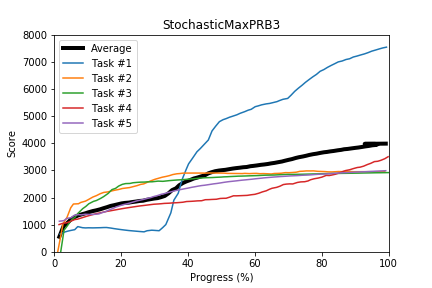
\includegraphics[width=\textwidth]{images/StochasticMaxPRB3.png}
    \end{subfigure}%
     ~
    \begin{subfigure}[t]{0.5\textwidth}
        \centering
        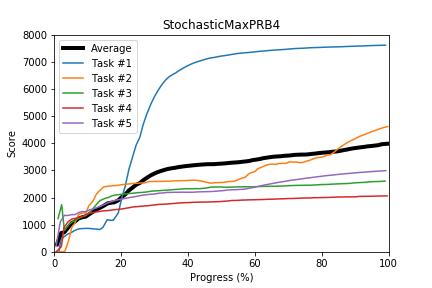
\includegraphics[width=\textwidth]{images/StochasticMaxPRB4.png}
    \end{subfigure}%
    \caption{Performance over time for Collection Threshold Methods}
        \label{fig:collection_performance}
\end{figure*}

\clearpage

\begin{figure*}[!ht]
	\begin{subfigure}[t]{0.5\textwidth}
        \centering
        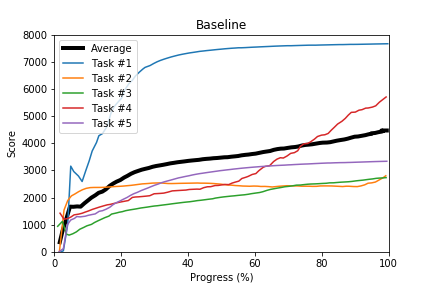
\includegraphics[width=\textwidth]{images/Baseline.png}
    \end{subfigure}%
    ~ 
    \begin{subfigure}[t]{0.5\textwidth}
        \centering
        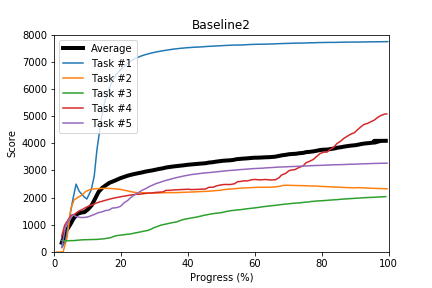
\includegraphics[width=\textwidth]{images/Baseline2.png}
    \end{subfigure}%

    \begin{subfigure}[t]{0.5\textwidth}
        \centering
        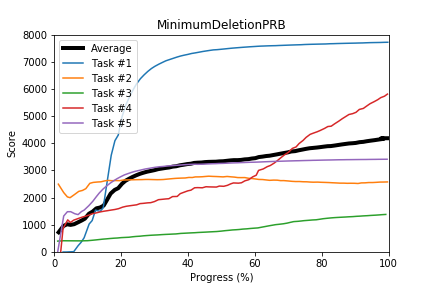
\includegraphics[width=\textwidth]{images/MinimumDeletionPRB.png}
    \end{subfigure}%
    ~
    \begin{subfigure}[t]{0.5\textwidth}
        \centering
        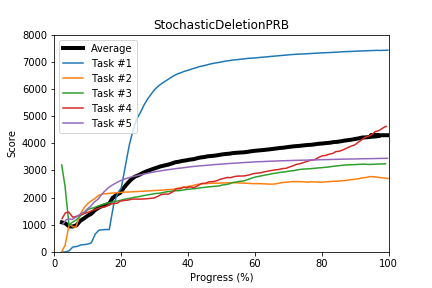
\includegraphics[width=\textwidth]{images/StochasticDeletionPRB.png}
    \end{subfigure}%
    
    \begin{subfigure}[t]{0.5\textwidth}
        \centering
        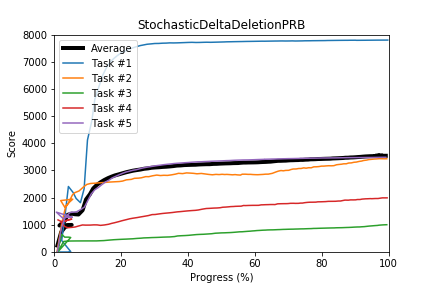
\includegraphics[width=\textwidth]{images/StochasticDeltaDeletionPRB.png}
    \end{subfigure}%
    \caption{Performance over time for Deletion Methods}
    \label{fig:deletion_performance}
\end{figure*}


\begin{figure*}[!ht]
    \begin{subfigure}[t]{0.5\textwidth}
        \centering
        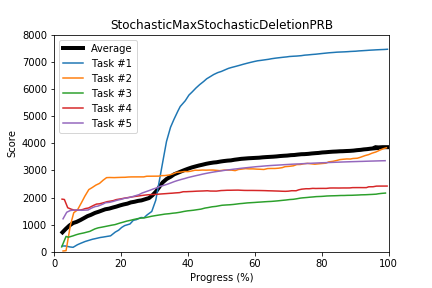
\includegraphics[width=\textwidth]{images/StochasticMaxStochasticDeletionPRB.png}
    \end{subfigure}%
    ~
    \begin{subfigure}[t]{0.5\textwidth}
        \centering
        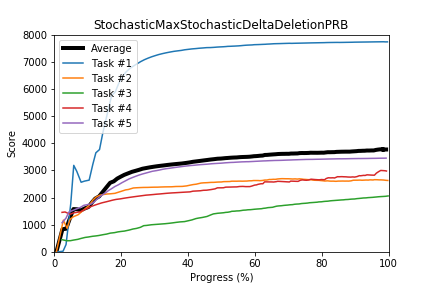
\includegraphics[width=\textwidth]{images/StochasticMaxStochasticDeltaDeletionPRB.png}
    \end{subfigure}%
    \caption{Performance over time for Stochastic Collection and Deletion Methods}
    \label{fig:combined_performance}
 
\end{figure*}

\end{document}
